\section{\tl{Linear Regression}}
\en{Linear Regression is a statistical method that aims to learn the relationship between dependent and independent variables. In our case, the goal is to study the shrinkage effect that AD and MCI have on brain size, and therefore to study it properly we need to isolate that effect. In order to do that, any effects that age, sex and different cranium sizes have, must be removed. Finding out the pattern between the brain size, which is the 145 ROI values, and the age the person has, as well as his/her gender and cranium size, is necessary if we want to remove it.

LR learns the trend between the independent variables (age, gender, cranium size) and the dependent variable (ROI volume), so calculating the difference from the computed trend values and the real values is called the residual values. We use those residual values as a means to recognize how intense the effect of the disease on the participant’s brain size is, since the other independent variables’ effects have been subtracted, meaning that if there was no effect, the trend between age, gender and cranium size would accurately predict the brain size and there would be no error. 

The model is trained on CN participants only, however all participants brain sizes are predicted using the trend line learned, to find out the difference between the real values and the predicted ones. We only keep the residual values, as they signify the difference from the trend line, which is equivalent to the intensity of the disease’s effect. 

The trend lines can be observed in the below figure for the ROI MUSE\_Volume\_48 which is translated to the left hippocampus area. It is clear that while the CN (green) population is centered around the x axis, meaning the brain size values are well predicted, the MCI population (blue) is lower than predicted, and the AD population (red) is much lower. This is expected, as the real brain size values are lower, since MCI and AD both cause a shrinkage of the brain.
\bigbreak
\begin{figure}[H]
    \centering
    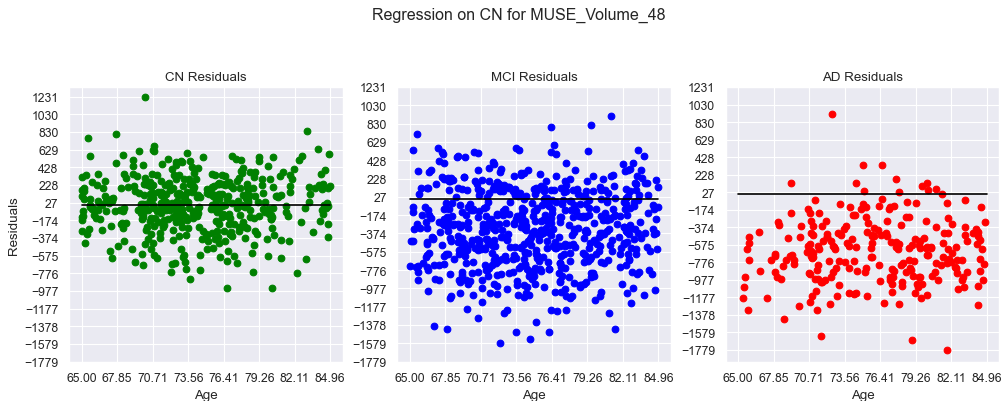
\includegraphics[width=\textwidth]{figures/Methodology/Linear_Regression.png}
    \caption{\en{Linear Regression on CN for MUSE\_Volume\_48}}
\end{figure}
\bigbreak

}